\documentclass{standalone}
\usepackage{tikz}
\usetikzlibrary{patterns, positioning}

\begin{document}
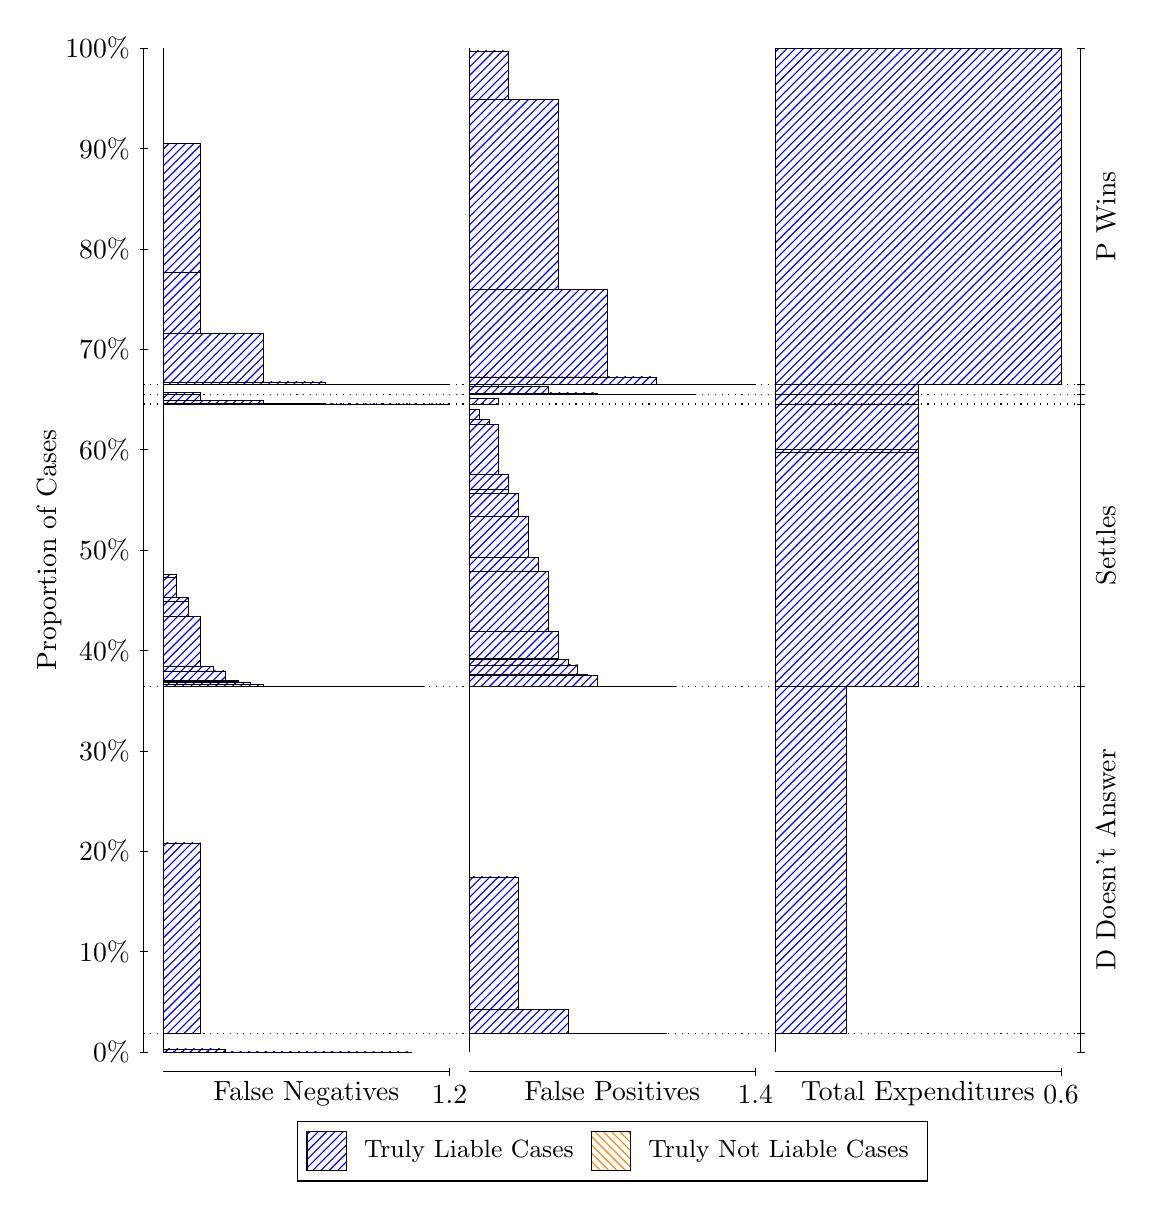
\begin{tikzpicture}
\draw[black, very thin] (1.5,1.75) -- (1.5,14.5);
\node[rotate=90, anchor=center] at (0.3, 8.125) {Proportion of Cases};
\draw[black, very thin] (1.45,1.75) -- (1.55,1.75);
\node[anchor=east] at (1.45, 1.75) {0\%};
\draw[black, very thin] (1.45,3.025) -- (1.55,3.025);
\node[anchor=east] at (1.45, 3.025) {10\%};
\draw[black, very thin] (1.45,4.3) -- (1.55,4.3);
\node[anchor=east] at (1.45, 4.3) {20\%};
\draw[black, very thin] (1.45,5.575) -- (1.55,5.575);
\node[anchor=east] at (1.45, 5.575) {30\%};
\draw[black, very thin] (1.45,6.85) -- (1.55,6.85);
\node[anchor=east] at (1.45, 6.85) {40\%};
\draw[black, very thin] (1.45,8.125) -- (1.55,8.125);
\node[anchor=east] at (1.45, 8.125) {50\%};
\draw[black, very thin] (1.45,9.4) -- (1.55,9.4);
\node[anchor=east] at (1.45, 9.4) {60\%};
\draw[black, very thin] (1.45,10.675) -- (1.55,10.675);
\node[anchor=east] at (1.45, 10.675) {70\%};
\draw[black, very thin] (1.45,11.95) -- (1.55,11.95);
\node[anchor=east] at (1.45, 11.95) {80\%};
\draw[black, very thin] (1.45,13.225) -- (1.55,13.225);
\node[anchor=east] at (1.45, 13.225) {90\%};
\draw[black, very thin] (1.45,14.5) -- (1.55,14.5);
\node[anchor=east] at (1.45, 14.5) {100\%};

\draw[black, very thin] (13.4,1.75) -- (13.4,14.5);
\draw[black, very thin] (13.35,1.75) -- (13.45,1.75);
\node[anchor=west] at (13.35, 1.75) {};
\draw[black, very thin] (13.35,1.9846) -- (13.45,1.9846);
\node[anchor=west] at (13.35, 1.9846) {};
\draw[black, very thin] (13.35,6.3934) -- (13.45,6.3934);
\node[anchor=west] at (13.35, 6.3934) {};
\draw[black, very thin] (13.35,9.9794) -- (13.45,9.9794);
\node[anchor=west] at (13.35, 9.9794) {};
\draw[black, very thin] (13.35,10.105) -- (13.45,10.105);
\node[anchor=west] at (13.35, 10.105) {};
\draw[black, very thin] (13.35,10.225) -- (13.45,10.225);
\node[anchor=west] at (13.35, 10.225) {};
\draw[black, very thin] (13.35,14.5) -- (13.45,14.5);
\node[anchor=west] at (13.35, 14.5) {};

\draw[black, very thin, pattern color=blue, pattern=north east lines] (1.75,1.75) rectangle (4.9094,1.75);
\draw[black, very thin, pattern color=blue, pattern=north east lines] (1.75,1.75) rectangle (4.1196,1.75);
\draw[black, very thin, pattern color=blue, pattern=north east lines] (1.75,1.75) rectangle (3.3297,1.7503);
\draw[black, very thin, pattern color=blue, pattern=north east lines] (1.75,1.7503) rectangle (2.5399,1.7884);
\draw[black, very thin, pattern color=orange, pattern=north west lines] (1.75,1.7884) rectangle (1.75,1.7884);
\draw[black, very thin, pattern color=blue, pattern=north east lines] (1.75,1.7884) rectangle (1.75,1.9846);
\draw[black, very thin, pattern color=blue, pattern=north east lines] (1.75,1.9846) rectangle (2.2239,4.4051);
\draw[black, very thin, pattern color=orange, pattern=north west lines] (1.75,4.4051) rectangle (1.75,4.4051);
\draw[black, very thin, pattern color=blue, pattern=north east lines] (1.75,4.4051) rectangle (1.75,6.3934);
\draw[black, very thin, pattern color=blue, pattern=north east lines] (1.75,6.3934) rectangle (5.0674,6.3934);
\draw[black, very thin, pattern color=blue, pattern=north east lines] (1.75,6.3934) rectangle (4.7514,6.3934);
\draw[black, very thin, pattern color=blue, pattern=north east lines] (1.75,6.3934) rectangle (4.4355,6.3934);
\draw[black, very thin, pattern color=blue, pattern=north east lines] (1.75,6.3934) rectangle (4.2775,6.3934);
\draw[black, very thin, pattern color=blue, pattern=north east lines] (1.75,6.3934) rectangle (4.1196,6.3934);
\draw[black, very thin, pattern color=blue, pattern=north east lines] (1.75,6.3934) rectangle (3.9616,6.3934);
\draw[black, very thin, pattern color=blue, pattern=north east lines] (1.75,6.3934) rectangle (3.8036,6.3934);
\draw[black, very thin, pattern color=blue, pattern=north east lines] (1.75,6.3934) rectangle (3.6457,6.3935);
\draw[black, very thin, pattern color=blue, pattern=north east lines] (1.75,6.3935) rectangle (3.4877,6.3936);
\draw[black, very thin, pattern color=blue, pattern=north east lines] (1.75,6.3936) rectangle (3.3297,6.3937);
\draw[black, very thin, pattern color=blue, pattern=north east lines] (1.75,6.3937) rectangle (3.1717,6.3951);
\draw[black, very thin, pattern color=blue, pattern=north east lines] (1.75,6.3951) rectangle (3.1717,6.3955);
\draw[black, very thin, pattern color=blue, pattern=north east lines] (1.75,6.3955) rectangle (3.0138,6.4212);
\draw[black, very thin, pattern color=blue, pattern=north east lines] (1.75,6.4212) rectangle (2.8558,6.446);
\draw[black, very thin, pattern color=blue, pattern=north east lines] (1.75,6.446) rectangle (2.6978,6.4615);
\draw[black, very thin, pattern color=blue, pattern=north east lines] (1.75,6.4615) rectangle (2.6978,6.4657);
\draw[black, very thin, pattern color=blue, pattern=north east lines] (1.75,6.4657) rectangle (2.5399,6.5891);
\draw[black, very thin, pattern color=blue, pattern=north east lines] (1.75,6.5891) rectangle (2.3819,6.6446);
\draw[black, very thin, pattern color=blue, pattern=north east lines] (1.75,6.6446) rectangle (2.3819,6.6515);
\draw[black, very thin, pattern color=blue, pattern=north east lines] (1.75,6.6515) rectangle (2.2239,7.284);
\draw[black, very thin, pattern color=blue, pattern=north east lines] (1.75,7.284) rectangle (2.0659,7.476);
\draw[black, very thin, pattern color=blue, pattern=north east lines] (1.75,7.476) rectangle (2.0659,7.5255);
\draw[black, very thin, pattern color=blue, pattern=north east lines] (1.75,7.5255) rectangle (1.908,7.7849);
\draw[black, very thin, pattern color=blue, pattern=north east lines] (1.75,7.7849) rectangle (1.908,7.8163);
\draw[black, very thin, pattern color=blue, pattern=north east lines] (1.75,7.8163) rectangle (1.75,7.8175);
\draw[black, very thin, pattern color=orange, pattern=north west lines] (1.75,7.8175) rectangle (1.75,7.8175);
\draw[black, very thin, pattern color=blue, pattern=north east lines] (1.75,7.8175) rectangle (1.75,9.9794);
\draw[black, very thin, pattern color=blue, pattern=north east lines] (1.75,9.9794) rectangle (5.3833,9.9794);
\draw[black, very thin, pattern color=blue, pattern=north east lines] (1.75,9.9794) rectangle (4.5935,9.9794);
\draw[black, very thin, pattern color=blue, pattern=north east lines] (1.75,9.9794) rectangle (3.8036,9.9848);
\draw[black, very thin, pattern color=blue, pattern=north east lines] (1.75,9.9848) rectangle (3.0138,10.03);
\draw[black, very thin, pattern color=blue, pattern=north east lines] (1.75,10.03) rectangle (2.2239,10.105);
\draw[black, very thin, pattern color=orange, pattern=north west lines] (1.75,10.105) rectangle (1.75,10.105);
\draw[black, very thin, pattern color=blue, pattern=north east lines] (1.75,10.105) rectangle (2.2239,10.13);
\draw[black, very thin, pattern color=orange, pattern=north west lines] (1.75,10.13) rectangle (1.75,10.13);
\draw[black, very thin, pattern color=blue, pattern=north east lines] (1.75,10.13) rectangle (1.75,10.225);
\draw[black, very thin, pattern color=blue, pattern=north east lines] (1.75,10.225) rectangle (5.3833,10.225);
\draw[black, very thin, pattern color=blue, pattern=north east lines] (1.75,10.225) rectangle (4.5935,10.225);
\draw[black, very thin, pattern color=blue, pattern=north east lines] (1.75,10.225) rectangle (3.8036,10.26);
\draw[black, very thin, pattern color=blue, pattern=north east lines] (1.75,10.26) rectangle (3.0138,10.876);
\draw[black, very thin, pattern color=blue, pattern=north east lines] (1.75,10.876) rectangle (2.2239,11.653);
\draw[black, very thin, pattern color=blue, pattern=north east lines] (1.75,11.653) rectangle (2.2239,13.29);
\draw[black, very thin, pattern color=orange, pattern=north west lines] (1.75,13.29) rectangle (1.75,13.29);
\draw[black, very thin, pattern color=blue, pattern=north east lines] (1.75,13.29) rectangle (1.75,14.5);
\draw[black, very thin, pattern color=orange, pattern=north west lines] (5.6333,1.75) rectangle (5.6333,1.75);
\draw[black, very thin, pattern color=blue, pattern=north east lines] (5.6333,1.75) rectangle (5.6333,1.9846);
\draw[black, very thin, pattern color=orange, pattern=north west lines] (5.6333,1.9846) rectangle (8.1391,1.9846);
\draw[black, very thin, pattern color=blue, pattern=north east lines] (5.6333,1.9846) rectangle (8.1391,1.9846);
\draw[black, very thin, pattern color=blue, pattern=north east lines] (5.6333,1.9846) rectangle (7.5126,1.9871);
\draw[black, very thin, pattern color=blue, pattern=north east lines] (5.6333,1.9871) rectangle (6.8862,2.2862);
\draw[black, very thin, pattern color=blue, pattern=north east lines] (5.6333,2.2862) rectangle (6.2598,3.9729);
\draw[black, very thin, pattern color=blue, pattern=north east lines] (5.6333,3.9729) rectangle (5.6333,6.3934);
\draw[black, very thin, pattern color=orange, pattern=north west lines] (5.6333,6.3934) rectangle (8.2644,6.3934);
\draw[black, very thin, pattern color=blue, pattern=north east lines] (5.6333,6.3934) rectangle (8.2644,6.3934);
\draw[black, very thin, pattern color=orange, pattern=north west lines] (5.6333,6.3934) rectangle (8.0138,6.3934);
\draw[black, very thin, pattern color=blue, pattern=north east lines] (5.6333,6.3934) rectangle (8.0138,6.3934);
\draw[black, very thin, pattern color=orange, pattern=north west lines] (5.6333,6.3934) rectangle (7.7632,6.3934);
\draw[black, very thin, pattern color=blue, pattern=north east lines] (5.6333,6.3934) rectangle (7.7632,6.3935);
\draw[black, very thin, pattern color=blue, pattern=north east lines] (5.6333,6.3935) rectangle (7.6379,6.3935);
\draw[black, very thin, pattern color=orange, pattern=north west lines] (5.6333,6.3935) rectangle (7.5126,6.3935);
\draw[black, very thin, pattern color=blue, pattern=north east lines] (5.6333,6.3935) rectangle (7.5126,6.3941);
\draw[black, very thin, pattern color=blue, pattern=north east lines] (5.6333,6.3941) rectangle (7.3874,6.3941);
\draw[black, very thin, pattern color=orange, pattern=north west lines] (5.6333,6.3941) rectangle (7.2621,6.3941);
\draw[black, very thin, pattern color=blue, pattern=north east lines] (5.6333,6.3941) rectangle (7.2621,6.5337);
\draw[black, very thin, pattern color=blue, pattern=north east lines] (5.6333,6.5337) rectangle (7.1368,6.5485);
\draw[black, very thin, pattern color=orange, pattern=north west lines] (5.6333,6.5485) rectangle (7.0115,6.5485);
\draw[black, very thin, pattern color=blue, pattern=north east lines] (5.6333,6.5485) rectangle (7.0115,6.6662);
\draw[black, very thin, pattern color=orange, pattern=north west lines] (5.6333,6.6662) rectangle (7.0115,6.6662);
\draw[black, very thin, pattern color=blue, pattern=north east lines] (5.6333,6.6662) rectangle (7.0115,6.6662);
\draw[black, very thin, pattern color=blue, pattern=north east lines] (5.6333,6.6662) rectangle (6.8862,6.7338);
\draw[black, very thin, pattern color=blue, pattern=north east lines] (5.6333,6.7338) rectangle (6.7609,6.7492);
\draw[black, very thin, pattern color=orange, pattern=north west lines] (5.6333,6.7492) rectangle (6.7609,6.7492);
\draw[black, very thin, pattern color=blue, pattern=north east lines] (5.6333,6.7492) rectangle (6.7609,7.0874);
\draw[black, very thin, pattern color=blue, pattern=north east lines] (5.6333,7.0874) rectangle (6.6356,7.8517);
\draw[black, very thin, pattern color=orange, pattern=north west lines] (5.6333,7.8517) rectangle (6.5103,7.8517);
\draw[black, very thin, pattern color=blue, pattern=north east lines] (5.6333,7.8517) rectangle (6.5103,8.0352);
\draw[black, very thin, pattern color=blue, pattern=north east lines] (5.6333,8.0352) rectangle (6.3851,8.5553);
\draw[black, very thin, pattern color=blue, pattern=north east lines] (5.6333,8.5553) rectangle (6.3851,8.5565);
\draw[black, very thin, pattern color=orange, pattern=north west lines] (5.6333,8.5565) rectangle (6.2598,8.5565);
\draw[black, very thin, pattern color=blue, pattern=north east lines] (5.6333,8.5565) rectangle (6.2598,8.8473);
\draw[black, very thin, pattern color=blue, pattern=north east lines] (5.6333,8.8473) rectangle (6.1345,8.8969);
\draw[black, very thin, pattern color=blue, pattern=north east lines] (5.6333,8.8969) rectangle (6.1345,9.0888);
\draw[black, very thin, pattern color=blue, pattern=north east lines] (5.6333,9.0888) rectangle (6.0092,9.7213);
\draw[black, very thin, pattern color=blue, pattern=north east lines] (5.6333,9.7213) rectangle (5.8839,9.7838);
\draw[black, very thin, pattern color=blue, pattern=north east lines] (5.6333,9.7838) rectangle (5.7586,9.9064);
\draw[black, very thin, pattern color=blue, pattern=north east lines] (5.6333,9.9064) rectangle (5.7586,9.9071);
\draw[black, very thin, pattern color=blue, pattern=north east lines] (5.6333,9.9071) rectangle (5.6333,9.9794);
\draw[black, very thin, pattern color=orange, pattern=north west lines] (5.6333,9.9794) rectangle (6.0092,9.9794);
\draw[black, very thin, pattern color=blue, pattern=north east lines] (5.6333,9.9794) rectangle (6.0092,10.055);
\draw[black, very thin, pattern color=blue, pattern=north east lines] (5.6333,10.055) rectangle (5.6333,10.105);
\draw[black, very thin, pattern color=orange, pattern=north west lines] (5.6333,10.105) rectangle (8.5149,10.105);
\draw[black, very thin, pattern color=blue, pattern=north east lines] (5.6333,10.105) rectangle (8.5149,10.105);
\draw[black, very thin, pattern color=blue, pattern=north east lines] (5.6333,10.105) rectangle (7.8885,10.106);
\draw[black, very thin, pattern color=blue, pattern=north east lines] (5.6333,10.106) rectangle (7.2621,10.119);
\draw[black, very thin, pattern color=blue, pattern=north east lines] (5.6333,10.119) rectangle (6.6356,10.201);
\draw[black, very thin, pattern color=blue, pattern=north east lines] (5.6333,10.201) rectangle (6.0092,10.225);
\draw[black, very thin, pattern color=orange, pattern=north west lines] (5.6333,10.225) rectangle (9.2667,10.225);
\draw[black, very thin, pattern color=blue, pattern=north east lines] (5.6333,10.225) rectangle (9.2667,10.225);
\draw[black, very thin, pattern color=orange, pattern=north west lines] (5.6333,10.225) rectangle (8.6402,10.225);
\draw[black, very thin, pattern color=blue, pattern=north east lines] (5.6333,10.225) rectangle (8.6402,10.226);
\draw[black, very thin, pattern color=orange, pattern=north west lines] (5.6333,10.226) rectangle (8.0138,10.226);
\draw[black, very thin, pattern color=blue, pattern=north east lines] (5.6333,10.226) rectangle (8.0138,10.324);
\draw[black, very thin, pattern color=orange, pattern=north west lines] (5.6333,10.324) rectangle (7.3874,10.324);
\draw[black, very thin, pattern color=blue, pattern=north east lines] (5.6333,10.324) rectangle (7.3874,11.435);
\draw[black, very thin, pattern color=orange, pattern=north west lines] (5.6333,11.435) rectangle (6.7609,11.435);
\draw[black, very thin, pattern color=blue, pattern=north east lines] (5.6333,11.435) rectangle (6.7609,13.849);
\draw[black, very thin, pattern color=blue, pattern=north east lines] (5.6333,13.849) rectangle (6.1345,14.465);
\draw[black, very thin, pattern color=blue, pattern=north east lines] (5.6333,14.465) rectangle (5.6333,14.5);
\draw[black, very thin, pattern color=orange, pattern=north west lines] (9.5167,1.75) rectangle (9.5167,1.75);
\draw[black, very thin, pattern color=blue, pattern=north east lines] (9.5167,1.75) rectangle (9.5167,1.9846);
\draw[black, very thin, pattern color=orange, pattern=north west lines] (9.5167,1.9846) rectangle (10.425,1.9846);
\draw[black, very thin, pattern color=blue, pattern=north east lines] (9.5167,1.9846) rectangle (10.425,6.3934);
\draw[black, very thin, pattern color=orange, pattern=north west lines] (9.5167,6.3934) rectangle (11.333,6.3934);
\draw[black, very thin, pattern color=blue, pattern=north east lines] (9.5167,6.3934) rectangle (11.333,9.3641);
\draw[black, very thin, pattern color=orange, pattern=north west lines] (9.5167,9.3641) rectangle (11.333,9.3641);
\draw[black, very thin, pattern color=blue, pattern=north east lines] (9.5167,9.3641) rectangle (11.333,9.3999);
\draw[black, very thin, pattern color=orange, pattern=north west lines] (9.5167,9.3999) rectangle (11.333,9.3999);
\draw[black, very thin, pattern color=blue, pattern=north east lines] (9.5167,9.3999) rectangle (11.333,9.9794);
\draw[black, very thin, pattern color=orange, pattern=north west lines] (9.5167,9.9794) rectangle (11.333,9.9794);
\draw[black, very thin, pattern color=blue, pattern=north east lines] (9.5167,9.9794) rectangle (11.333,10.105);
\draw[black, very thin, pattern color=orange, pattern=north west lines] (9.5167,10.105) rectangle (11.333,10.105);
\draw[black, very thin, pattern color=blue, pattern=north east lines] (9.5167,10.105) rectangle (11.333,10.225);
\draw[black, very thin, pattern color=orange, pattern=north west lines] (9.5167,10.225) rectangle (13.15,10.225);
\draw[black, very thin, pattern color=blue, pattern=north east lines] (9.5167,10.225) rectangle (13.15,14.5);
\draw[black, dotted] (1.5,1.9846) -- (13.4,1.9846);
\draw[black, dotted] (1.5,6.3934) -- (13.4,6.3934);
\draw[black, dotted] (1.5,9.9794) -- (13.4,9.9794);
\draw[black, dotted] (1.5,10.105) -- (13.4,10.105);
\draw[black, dotted] (1.5,10.225) -- (13.4,10.225);
\draw[black, very thin] (1.75,1.5) -- (5.3833,1.5);
\node[anchor=north] at (3.5667, 1.5) {False Negatives};
\draw[black, very thin] (5.3833,1.45) -- (5.3833,1.55);
\node[anchor=north] at (5.3833, 1.45) {1.2};

\draw[black, very thin] (5.6333,1.5) -- (9.2667,1.5);
\node[anchor=north] at (7.45, 1.5) {False Positives};
\draw[black, very thin] (9.2667,1.45) -- (9.2667,1.55);
\node[anchor=north] at (9.2667, 1.45) {1.4};

\draw[black, very thin] (9.5167,1.5) -- (13.15,1.5);
\node[anchor=north] at (11.333, 1.5) {Total Expenditures};
\draw[black, very thin] (13.15,1.45) -- (13.15,1.55);
\node[anchor=north] at (13.15, 1.45) {0.6};


\node[black, centered, rotate=90] at (13.72, 4.189) {D Doesn't Answer};
\node[black, centered, rotate=90] at (13.72, 8.1864) {Settles};


\node[black, centered, rotate=90] at (13.72, 12.362) {P Wins};

\draw (7.449999999999999,1.5) node[draw=none] (baseCoordinate) {};
\begin{scope}[align=center]
        \matrix[scale=0.5, draw=black, below=0.5cm of baseCoordinate, nodes={draw}, column sep=0.1cm]{
            \node[rectangle, draw, minimum width=0.5cm, minimum height=0.5cm, pattern=north east lines, pattern color=blue] {}; &
            \node[draw=none, font=\small] (B) {Truly Liable Cases}; &
            \node[rectangle, draw, minimum width=0.5cm, minimum height=0.5cm, pattern=north west lines, pattern color=orange] {}; &
            \node[draw=none, font=\small] (B) {Truly Not Liable Cases}; \\
            };
\end{scope}

\end{tikzpicture}
\end{document}